\documentclass[11pt]{article}
\usepackage[margin=1in]{geometry}          
\usepackage{graphicx}
\usepackage{amsthm, amsmath, amssymb}
\usepackage{setspace}\onehalfspacing
\usepackage[loose,nice]{units}
\usepackage{array}
\usepackage[super]{nth}
\usepackage{graphicx}
\usepackage{float}
\usepackage{subcaption}
\usepackage{mathtools}
\usepackage[displaymath, mathlines]{lineno}
\usepackage{natbib}
\usepackage[all]{nowidow}
\usepackage{wrapfig}
\newenvironment{conditions}
  {\par\vspace{\abovedisplayskip}\noindent\begin{tabular}{>{$}l<{$} @{${}={}$} l}}
  {\end{tabular}\par\vspace{\belowdisplayskip}}
\newcommand{\R}{\mathbb{R}}  
 
\author{
	Dr. Yoav Ram
	\and
	Saar Egozi
}
\date{Autumn 2019}
 
\begin{document}
\begin{titlepage}
\centering

\vspace{4cm}

{\Large Research Proposal}

\vspace{2cm}

{\LARGE\bfseries Prestige as a Driving Force in Cultural Transmission}

\vspace{2cm}

{\large\bfseries Saar Egozi}

\vspace{1cm}

{\large Mentored by Yoav Ram}

\vspace{2cm}

\vfill

{\large Efi Arazi School of Computer Science, IDC Herzliya}

\vspace{1cm}

{\itshape \today}

{\large saartk@gmail.com}
\end{titlepage}

\clearpage
\renewcommand\linenumberfont{\normalfont\small\sffamily}
%\linenumbers
%\modulolinenumbers[2]
\section*{Introduction}

%use different citing as needed, usually at start or end of sentence
%use positive approach with the reader, do not encourage conflict with him
% use thesaurus and morfix for uncomfortable words
% ascribe each sentence with its topic, then group same topics together
% each paragraph should have a goal
% model to copy from is role-model
% replace "in this study" with "here"



%Introduction:
% 1 - what is cultural transmission
% 2 - where in nature we see it (examples)
% 3 - compare and contrast with genetic transmission
% 4 - transmission biases - what are they, what are the types
% 5 - prestige bias - what is it, why is it different than the rest
% 6 - examples/ support for the prestige bias. (why is it relevant now?)

% what is cultural transmission, and its not only in humans
Cultural transmission is the way individuals inherit cultural traits from one another, typically via learning or copying. %what is cultural transmission
 It is common in humans \citep[pg. 3]{transmissionVectorsBook}, and in primates, such as chimpanzees \citep{chimpsPrestige, chimpsCopy}. %appears in humans and primates
 The common cultural traits in humans are behavioural patterns, like personalities and habits, transmitted via observations and verbal discussions \citep{dualEvolution}. %how it is transmitted in humans
 They suggest that cultural learning may be particular to humans, but \citet{elepahntsRepo} suggest that it appears in other mammals, such as elephants. %not only in humans, in elephants too
 They demonstrated that: 
 \begin{quote}
	   ... the possession of enhanced discriminatory abilities by the oldest individual in a group can influence the social knowledge of the group as a whole.
 \end{quote}
 They showed that once a matriarch is removed from the group, the group's survival instincts are inferior. %the conclusion of the study
 They did that by playing audio recordings of African elephants, and showed that groups with a matriarch recognise and react better to hostile or friendly calls than the groups without one. % what was the experiment.
It appears that cultural transmission appears in other species, which are simpler than mammals, such as \textit{Drosophila}. % cultural transmission in flies
\citet{fliesPaper} show that oviposition site choice in fruit flies is culturally transmitted. % an example study for the flies
They showed that flies without experience in choosing sites, after spending some time with experienced flies, chose the same type of site without directly observing this behaviour. %explanation of the experiment
\citet{fliesPaper} mention that the how the information is transferred is still an open question, but suggest that the flies may use olfactory cues, like other animals, such as rodents and bees.\\ %how they are transmitted

%the differences and similarities between cultural and genetic transmission 
It appears cultural transmission is similar to genetic transmission in many ways, while very different in others. %general paragraph statement - cultural is similar but different from genetic
Similar to genetic transmission, the effects of culturally transmitted traits can be physiological rather than behavioural, and transmitted from parents to offspring.%similarity - cultural may be physiological
 For example, parents can teach their children to be strong or tall, within some biological limits, when they tell them to eat healthy and engage in physical exercises. %support the claim of physiological affects
Contrary to genetic transmission, the sources of the traits can be teachers, celebrities, coaches, the media, or any stranger that comes in contact with them. %contrast - the source of transmission
 Cultural transmission can be vertical, where parents transmit to their children, but also oblique, where other adults transmit traits to children (not their own). %oblique
  Horizontal transmission is also possible, where peers transmit traits to one another. %horizontal
   Lastly, vertical transmission in the opposite direction is possible too, where parents copy traits from their children \citep{transmissionVectorsBook, transmissionVectors}. %opposite vertical
In addition, even when a cultural trait is disfavoured by natural selection, it still may spread across a population given transmission biases \citep[Ch. 8 pg. 279]{evolutionBook}.\\ %another  try to use positive

%transmission biases - what they are, what are the types.
Transmission bias occurs when a trait has a disproportionate probability to be transmitted.  %what is a transmission bias
For example, \citet{wtfGene} showed that there are genes of yeast (called \textit{wtf genes}) that bias their transmission to the gametes. %example for transmission bias in genetics
They secrete a long life expectancy poison, together with a short life expectancy antidote, so a gamete without the gene will perish (the poison will outlive the antidote). %how the bias is made
Transmission biases, though exist in genetic transmission, are probably more common in cultural transmission. %transmission in cultural
 \citet{strategiesPaper} suggest that success biased social transmission contribute more to the general success of the population than individual learning. %success bias is better than individual learning
 They conducted a tournament for developing learning strategies of a population, where each participant need to suggest a strategy. % the tournament description
 Each strategy must define when individuals should observe and copy from others, and when to engage in individual learning. % continue of description
 The best strategies contained a high percentage of social learning, even when the error when copying was as high as almost 0.5. %the results
In addition to \citet{strategiesPaper}, \citet{complexityPaper} define different types of transmission biases based on success. %there are success biases
They define several types of role model choosing methods, all assuming that the copier correctly identifies the successful ones. %support for success bias 
Both studies assume that individuals can successfully evaluate successful individuals.
\citet[Ch. 5]{evolutionBook} suggest that the evaluation of success can be divided into three groups - \textit{direct bias}, \textit{indirect bias} and \textit{frequency-dependant bias}. %the types of cultural biases
A direct bias is when a variation of a trait is more attractive than others, and is evaluated by \textit{directly} testing the variation of the trait. %what is direct bias
For example, an individual observing a Ping-Pong match between two others can try both paddle grips it observed, and decide what grip is better for it. %an example for direct
An indirect bias is when an individual uses the value of one trait to determine the attractiveness of another, so it \textit{indirectly} evaluates the attractiveness of the trait. %what is indirect bias
Following the example, a bystander could copy the paddle grip of the more successful Ping-Pong player (by keeping score for example). %example for indirect bias
A frequency-dependant bias is when an offspring has a probability to copy a variant of the trait that is nonlinear to the trait's frequency in the parent's generation. %what is frequency dependant bias
Continuing with the example, an individual copying the grip most players use, is affected by the \textit{frequency} this of this grip in the population.\\ %example for frequency dependant
 
%prestige bias - what is it, what's missing
Prestige refers to a good reputation or high-esteem, therefore does not directly signify success (although it may imply it), making it an \textit{indirect bias}. %what is prestige
Both \citet[Ch. 8]{evolutionBook} and \citet{complexityPaper} claim that prestige biases are probably more common in humans than success biases. %prestige is more common
\citet[Ch. 8]{evolutionBook} add that maladaptive traits may spread widely in a population, if the indirect bias is strong enough. % prestige can spread maladaptive traits
They claim the bias could lead to a \textit{runaway process}, caused by a cultural equivalent of \textit{sexual selection} \citep{sexualSelectionBook}.
On the other hand, \citet{henrichBroesch} claim that prestige biases, over generations, can lead to cultural adaptations. %prestige can spread adaptive traits 
Hence prestige can cause a maladaptive trait to spread in the population, but can also accelerate the spread of adaptive traits. % prestige both good and bad
Prestige bias is mentioned in the literature many times, but rarely modelled. % current studies don't define prestige good enough
\citet{evolutionBook} have modelled the prestige bias, but didn't include the effects the copiers of a role model has on the probability of other individuals to choose the same role model.\\ % describe what influence is
This effect is similar to conformity, which is usually modelled as a different bias.
\citet{evolutionBook} have suggested a model for \textit{frequency dependant biases}, which include conformity bias.
\textit{Conformist learning} (imitating locally common behaviours) is a known bias in cultural transmission \citep{conformism}.
Our new component, \textit{influence}, is assigned to a role model, contrary to conformity, which refers to the probability of a specific variation of a trait.
If we define the copying of a role model $i$ as a trait itself, then \textit{influence} falls under the category of conformity.
We believe that prestige bias is a combination of the \textit{indirect bias} as \citet{evolutionBook} suggest, and of the \textit{influence} a role model has on the population.
\textbf{The goal of this study is to define a more realistic model for prestige bias and analyse the dynamics of the population it causes}. %the goal of the study - defining prestige bias 
Today, due to social media, it is easier than ever to estimate the influence individuals have over others, therefore it is probably a major part of our decision-making process.  
We want to create a model that better fits reality, and simulate scenarios that better mimic cultural transmission dynamics.
With a more accurate model of prestige bias, we can understand better how cultural traits are transmitted, and why.
Moreover, we could explain better the cause for the spread of maladaptive traits, or the acceleration of adaptive traits in reality.

\section*{Research plan}
 \paragraph{General model.} Consider a large population with $N$ individuals, with non-overlapping generations. %general description of the models
  Every individual has two types of traits - \textit{role model traits}, and \textit{copier traits}. % groups of traits
    \textbf{Role model traits} are composed of: an \textit{indicator trait}, which affects the attractiveness of the role model; % short explanation of indicator
   \textit{indirectly biased trait}, which may affect the fitness of the role model, but doesn't affect its attractiveness; % short explanation of indirect trait
   and \textit{influence}, which is the number of other copiers that chose this role model, weighted by their own \textit{influence}, and also affects the role model's attractiveness. %short explanation of influence
   For example, an amateur hunter who wants to choose a role model to copy, cannot follow all the hunters in its village, because it is impractical. % an example of a hunter
   The amateur needs another indication that signals success, for example: the quality or the size of the spear that a role model carries. % an example for the indicator
   However, the amateur understands that the spear isn't the sole source of the hunter's success, only implies it, and therefore he copies other behaviours too: face paint, schedule, and other rituals the chosen role model performs. %example of indirect trait
   The spear's features (quality or size) are therefore \textit{indicator traits}, while the other rituals copied are \textit{indirectly biased traits} (indirect traits in short). % explaining the example
   We also assume a hunter copied by other prestigious hunters, is more valued than a hunter copied by the same number of amateur hunters. %weighted influence
   Each copier (naive individual) evaluates the prestige of each available role model by estimating its indicator trait and influence values and chooses one based on it.  % how the prestige is calculated
   Transmission is based on cultural biases only. Natural selection is not taken into consideration in this model.
   The prestige score of role model $i$ out of $N$ is:
   \begin{equation}\label{naive prestige}
   	P_i = A_i + R_i,
   \end{equation}
   where $A_i$ is the indicator trait value of role model $i$, $A_i \in \R$, and  $R_i$ is the influence value of the role model, given by: %equation's explanation
   \begin{equation} \label{influence definition}
   R_i = 1 +\sum\limits_{j=1}^{k} R_j,
   \end{equation}
   where $k$ is the number of current copiers of role model $i$, and $R_i \ge 1$ (the influence of a role model with no copiers is 1, to avoid nullification of the recursive equation).
   The equation is always satisfied because there cannot be any cycles in the copying order: 
   assume individual $j$ copied from individual $i$, by the model's design, it means individual $i$ didn't copy individual $j$, nor any descendant of it,
    because $j$ doesn't have any copiers of its own at the moment of copying from $i$.
   Equation (\ref{influence definition}) describes a solution for a weighted ranking problem, resembling the PageRank algorithm \citep{pageRank}.\\

   Equation (\ref{naive prestige}) implies that every copier $j$ evaluates role model's $i$ prestige equally. %why the weights are needed
   We assume each copier values the indicator trait and the influence trait differently - some hunters may be more impressed by spear size, regardless of number of copiers. % 
   Therefore, naive individuals are born with \textbf{copier traits}, to differentiate their estimation process from one another: % introducing copier traits
   \textit{indicator weight} and \textit{influence weight} are traits that control the importance of the indicator and influence traits for copier $j$.
   $P_{ij}$ is the prestige score of role model $i$, evaluated by copier $j$ such that: % weights as copier traits
   \begin{equation}\label{weighted prestige}
   	P_{ij} = \alpha_j A_i + (1-\alpha_j) R_i,
   \end{equation}
   where $\alpha_j$ and  $1-\alpha_j$ are the weights of the indicator and influence traits ,respectively, and $\alpha_j \in [0,1]$.
   Equation (\ref{weighted prestige}) implies that the higher the indicator and influence values are, the more prestigious the role model. % explain why higher indicator is higher prestige
   However, a higher indicator doesn't always mean higher prestige: a spear the size of the moon is impractical, therefore we define an ideal value for the indicator trait. % why we need preference trait
   Here, we keep the assumption that high influence is always better, though in reality that isn't always the case. %influence is the higher the better
   The optimal indicator value is another copier trait, and could be homogenous or individually assigned. We call it the \textit{preference trait}, $\hat{A}_j$: %introducing preference trait
   \begin{equation} \label{preferenced prestige}
   P_{ij} = \alpha_j \beta(A_i,\hat{A}_j) + (1-\alpha_j) R_i
   \end{equation}
   where $\beta$ is the \textit{bias function}, such that: $\beta(A,\hat{A})=b*e^{\frac{-(A - \hat{A})^2}{2J}}$, and $J,b$ are parameters to control the strength of the bias. %explanation
    In our models the preference trait is homogenous: i.e all the copiers have the same preference trait value, so without loss of generality, we define $\hat{A}_j=1$ for every $j$. % preference trait is homogenous
   The closer the indicator value of the role model to the copier's preference trait, the greater the bias.\\
   Equation (\ref{preferenced prestige}) implies that every copier evaluates the traits equally and accurately. %the assumption of no errors
   In real life, not all copiers have the same access to the role models' spears. %why its not realistic
   Moreover, even given access to measure the spears' sizes, it would be very time consuming, so amateur copiers need to evaluate the spears by observing them. %using the example
   Therefore, we assume each copier is capable of different levels of accuracy, so each copier is born with its own error values for estimating indicator values $e_A$ (we assume influence can be measured easily, therefore it is accurate):
    \begin{equation} \label{prestige eq}
   P_{ij} = \alpha_j \beta((A_i+e_{jA}),\hat{A}) + (1-\alpha_j) R_i
   \end{equation}
   This model is inspired by the model \citet[Ch. 8][pg. 243-244]{evolutionBook} suggest for an indirect bias.\\ %inspired by boyd and richerson
   After evaluating the prestige scores of all available role models, the copier chooses a role model to copy with a probability $Pr(j | i)$ such that:
   \begin{equation}\label{prestige probability}
    P_r(j | i) = \frac{P_{ij}}{\sum\limits_{i=1}^{N} P_{ij}}
   \end{equation}
    Once a role model is chosen, the indicator and indirect traits $A_i,B_i$ are transmitted with errors: %transmission method
   \begin{equation}
   	(A_j,B_j) = (A_i+e_{jA},B_i+e_{jB}),
   \end{equation}
   where $j$ is the index of the copier that chose role model $i$ as its role model, $B \in \R$, and $e_B$ is the indirect trait error.
   We assume influence cannot be transmitted, only acquired by being copied by others. %influence is not transmitted
   In the first generation, the indicator and indirect traits are drawn from a 2D normal distribution, with a correlation of $\chi$.
   The errors are drawn from a 2D normal distribution as well, for each naive copier born, with $\zeta$ correlation, and scaled down by the \textit{error scale} parameter $\eta$.\\  %error scale
   Once all the copiers are informed they replace the role models' generation, and a new naive generation of copiers is born. 

   \paragraph{Aim 1: strengthening our alternative transmission mode: the random choice transmission.} 
   To support our suggested model, we first compare it with \citet{evolutionBook} indirect bias model to show that it achieves similar results. %why we compare
   The most significant difference between our model and theirs, is the additional influence trait, and the transmission mode. % the major differences
   In their model, \citet{evolutionBook} suggest a transmission mode called \textit{blending transmission}. %introducing the blending transmission
   The concept of the blending mode is the following: each naive individual copies an average of all the role models' traits, weighted by their prestige score, instead of choosing one at random.  %explaining the blending model
   In their model, \citet{evolutionBook} use two different bias functions: one for each trait, and both take only the preference trait and the indicator trait as parameters. % bias functions
   This results in two prestige scores for each role model, distinguished by a slight magnitude difference. % 2 bias functions
   Each of the traits is then transmitted separately, depending only on its respective score. %transmitted separately
   In addition, the prestige score is modified by a basic social rank, that is drawn randomly at birth. %social rank
   To maintain minimum difference, we assume indicator weight $\alpha_j=0$ for every copier $j$, to eliminate the influence value in this model.\\ %no influence
   Including the basic social rank, in this comparison model, the prestige evaluation equation is
   \begin{equation}\label{prestige with social rank}
    	P_{ij} = \tau_i + \beta((A_i+e_{jA}),\hat{A}),
   \end{equation}
   where $\tau_i$ is the social rank of role model $i$, drawn at random from the interval $[0,\beta((A_i+e_{jA}),\hat{A})]$, to avoid overshadowing the indicator trait value significance.
   We assume generations are non-overlapping, and transmission is oblique only. %model's rules
   The expected value of a trait $X$ (either indicator or indirect) when copier $i$ is choosing a model is: $E[X] = \sum\limits_{j=1}^{n} A_j P_{ij}$, which is the equation for the blending mode transmission \citep[eq. 8.9, 8.10]{evolutionBook}. % why it is similar to the blending mode
   The population in both models is finite, but is supposedly large enough so that $Var(X)$ is small. %population is finite, so law of large number is not exact
   
   \paragraph*{Preliminary results.}
   We compare our suggested transmission mode, the random choice mode (eq.\ref{prestige probability}), with the blending transmission mode \citet[eq. 8.9, 8.10]{evolutionBook} have suggested. %the results in a sentence
We tested several cases, the most interesting being those with a high correlation value between indicator and indirect trait values. %several scenarios
Figure \ref{randomVSblendingFigSingle} shows a single simulation with high initial traits correlation $\chi = 0.9$, relatively small population size, $N=1000$, over $1000$ generations. Starting population is the same in both simulations of transmission modes (blending and random choice).\\

  \begin{wrapfigure}{l}{0.5\textwidth}
  \begin{subfigure}[b]{\linewidth}
  \caption{Indicator trait evolution}
    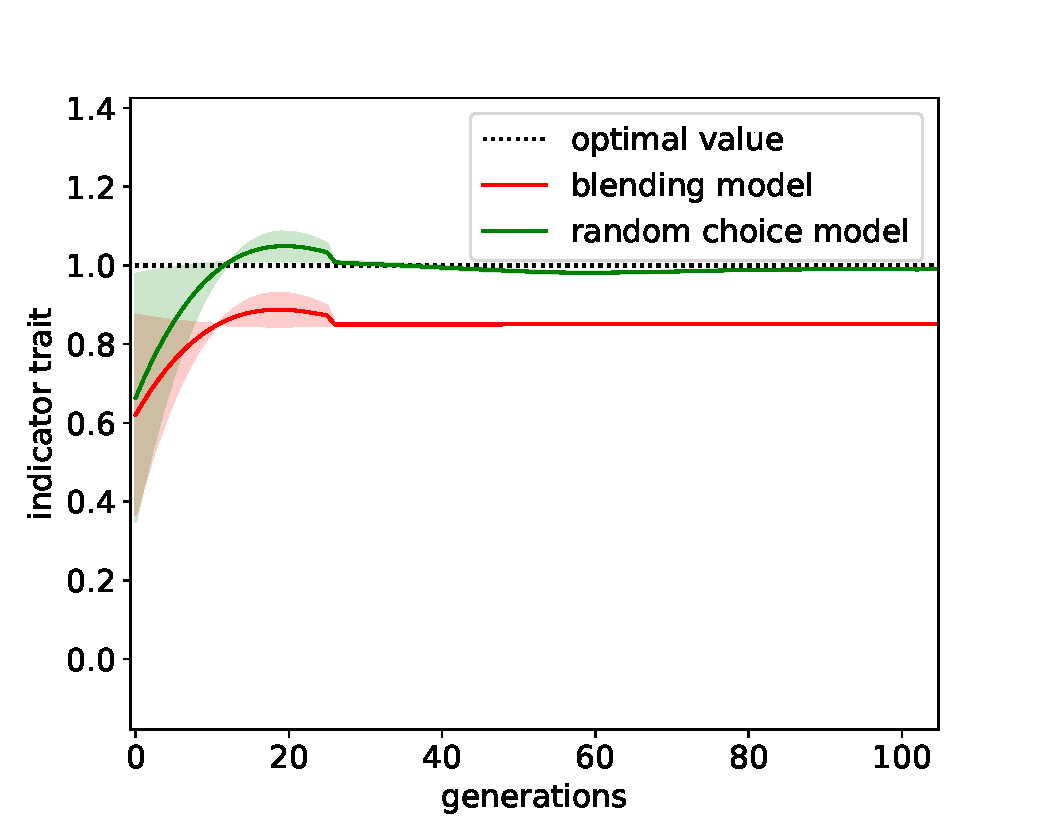
\includegraphics[width=\linewidth]{../../graphs/blending-vs-random/indicator_single_1000x1000_09Corr.pdf}
  \end{subfigure}
  \begin{subfigure}[b]{\linewidth}
  \caption{Indirectly biased trait evolution}
    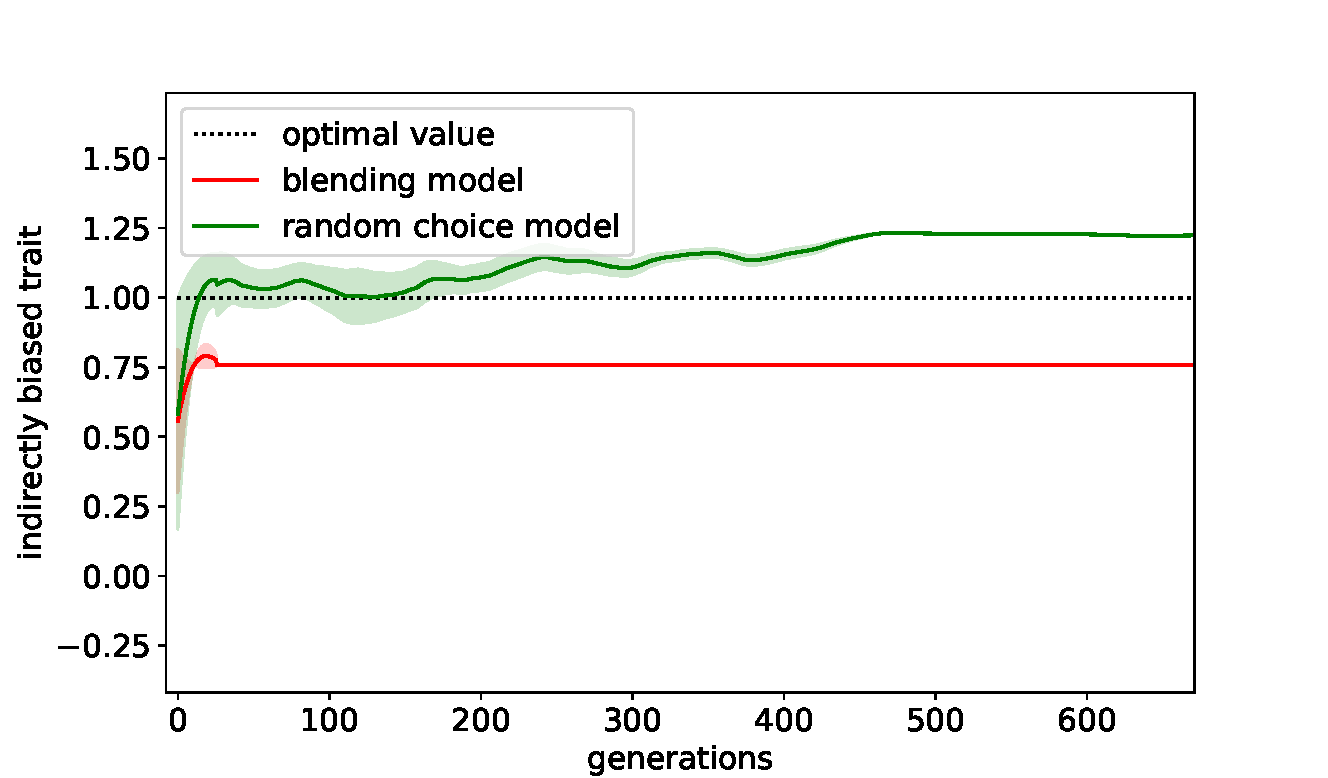
\includegraphics[width=\linewidth]{../../graphs/blending-vs-random/indirect_single_1000x1000_09Corr.pdf}
  \end{subfigure}
  \caption{Blending vs Random Choice model. Faded is standard deviation. Population size 1000. Single simulation, initial trait values chosen from a 2D normal distribution with a 0.9 correlation. Starting population the same in both realisations. Faded area represents standard deviation}
  \label{randomVSblendingFigSingle}
\end{wrapfigure}

 We see that both transmission modes result in a mean indicator value that is converging towards the optimal value in the beginning. % mean indicator close to optimal
 However, when using the blending transmission mode the population becomes homogenous in a very early stage, therefore probably preventing the mean value to converge to the optimum. % blending can't reach optimum
In both transmission modes the mean indirect trait value doesn't converge to the optimal indicator value, even though the initial correlation between the traits was very high. % correlation isn't enough
When using the blending transmission the variance is again converging to zero very fast, but in the random choice transmission the mean value becomes stable much later.\\ %blending is less flexible

\begin{wrapfigure}{l}{0.5\textwidth}
  \begin{subfigure}[b]{\linewidth}
  \caption{Indicator trait evolution}
    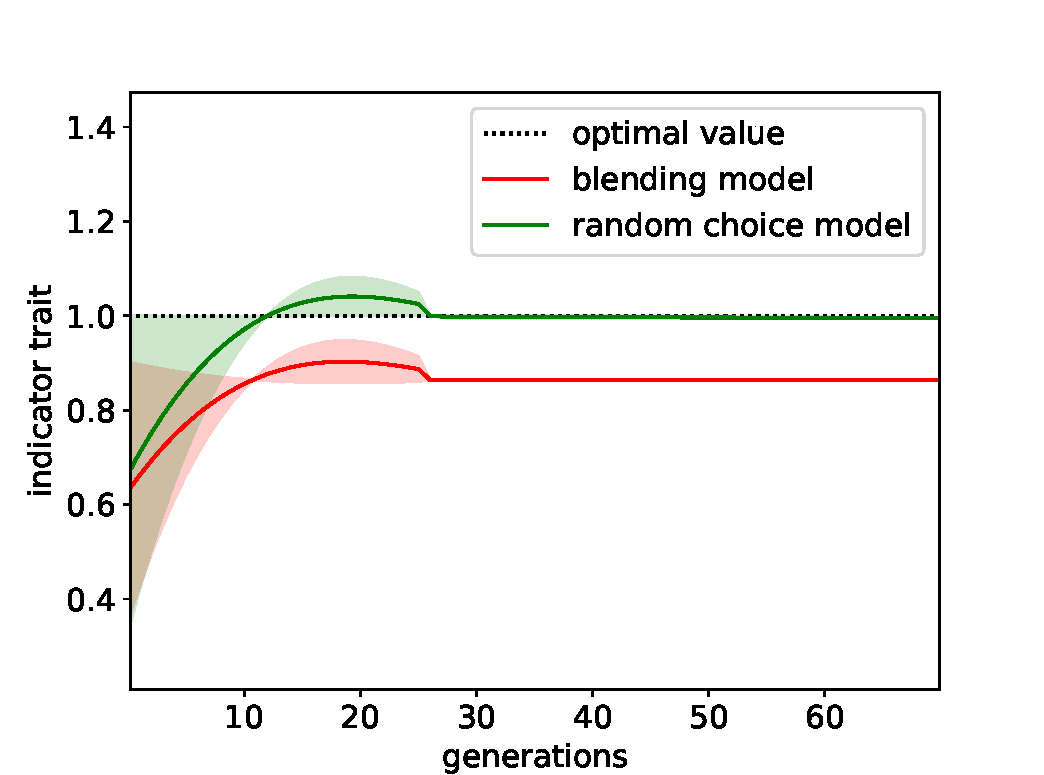
\includegraphics[width=\linewidth]{../../graphs/blending-vs-random/indicator_21_diffInit_1000x1000_09Corr.pdf}
  \end{subfigure}
  \begin{subfigure}[b]{\linewidth}
  \caption{Indirectly biased trait evolution}
    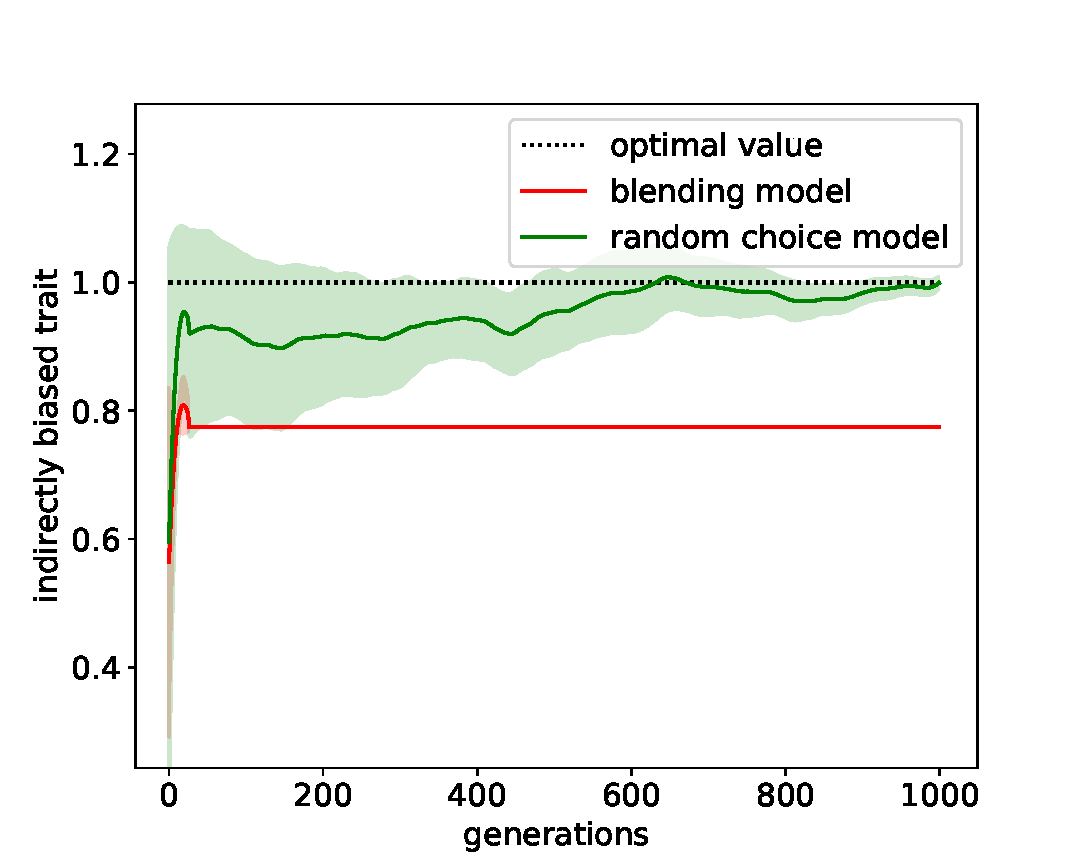
\includegraphics[width=\linewidth]{../../graphs/blending-vs-random/indirect_21_diffInit_1000x1000_09Corr.pdf}
  \end{subfigure}
  \caption{Blending vs Random Choice model. Population size 1000. Mean values of 20 simulations, initial trait values chosen from a 2D normal distribution with a 0.9 correlation (chosen randomly in each simulation). Faded area represents mean of standard deviation}
  \label{randomVSblendingFigMultiple}
\end{wrapfigure}

When calculating the mean values of 20 simulations, with the same parameters, the results are a bit different, as seen in Figure \ref{randomVSblendingFigMultiple}.\\
We see that when using either of the transmission modes, the mean indicator values both converge to the optimal value (random choice converging to a closer value), and the variance is converging to zero in a very early stage. % indicators in multiple runs
The difference between the two transmission modes when observing the indirect value is more prominent. %there is a difference in indirect
When using the blending mode the variance is still converging to zero very fast, and the stable value of the indirect trait doesn't reach the optimal indicator value, nor the mean indicator value. %blending didn't reach it
When using the random choice model, we see that the variance is relatively large at the beginning, and slowly converging to zero towards the end of the simulation. %random choice did
We also see that the mean indirect value converges to the optimal indicator value, meaning that the initial correlation sufficed when using this transmission mode.
We believe that the variance of the blending mode will not converge to zero as quickly only if the error scale we use is considerably larger.
By the definition of the blending mode (a weighted average), we believe that even when injecting a single optimal role model each generation, the mean indicator value will not reach the optimal value as fast as in the random choice mode. \\ %also to the indicator value
   

 \paragraph*{Aim 2: creating a basic yet realistic model that includes influence, and analyse the dynamics in the population.}\label{basic model}
 We believe that influence may have significant effects on the mean value of the indicator and indirect traits in the population, even in its most basic form.
  Therefore we define a simple version of our model where we limit the transmission to oblique transmission only (and the generations are still discrete). %general rules - oblique and discrete
  This model has several variations: \textbf{homogenous weights}, where every individual has the same weights $\alpha$; %model variations
   \textbf{random weights}, where every individual has (different) random weights $\alpha_j$;
    \textbf{transmitted correlated weights}, where the weights are correlated to the traits of the first role models' generation, and the copier copies the weights of the role model (accurately) $\alpha_j = \alpha_i$. %model variations
  The transmission mode we use is the random choice transmission, so we can keep track who copied from whom. %transmission mode - random choice
  Since generations are discrete, influence is "shallow", meaning it is equal to the number of copiers. %shallow influence
  For every role model evaluated by each of the copiers, we count the number of copiers who chose this role model, and calculate the score accordingly. %evaluation
  The evaluation process is according to equation (\ref{prestige eq}). %evaluation continue
  We expect that the homogenous weights variation will increase the variance both indicator and indirect traits, compared to the atrophied version of our model described in step 1.
  We believe that the higher the influence weight will be, the higher the variance of both traits will be.
  We also expect that the when the variance of the traits will converge to zero, the maximum influence value will decrease as well, because the role models will have similar indicator values, therefore similar prestige scores.
    We believe that the variation in reality isn't homogenous, therefore we want to compare the opposite (random weights) to see if the results are more reasonable.
  We assume that the mean and variance of both traits in the random weights variation will be similar to homogenous equal weights, $\alpha=0.5$.
  The last variation, the transmitted correlated weights, is probably the most realistic scenario: when an individual is valued for his remarkable indicator value, he will probably value it more in others.
  We expect that when the correlation is high, the mean influence weight will converge to 0, or decrease significantly between generations.\\
  
  \paragraph*{Preliminary results.}
  We ran 35 simulations, population size $N=5000$, indicator-indirect traits correlation $\chi=0.9$, with different starting generation each simulation, and error scale $\eta=100$.
  The model variation we tested is the random weights variation, and the results are shown in Figure \ref{basic influence fig}.
  We see several differences between this model and the variation without any influence: 
  The variance of both indicator and indirect traits is larger than before, and don't converge to zero;
  The indirect trait mean doesn't converge to the optimal indicator value, and even drifts away in the later generations;
  The indirect trait mean is stabler than the previous model using the random choice transmission mode; 
  The indicator mean value takes longer to converge to the optimal value (the ~200th generation vs. the ~30th).
  These results could be caused by both the larger population size $N$, and smaller error scale $\eta$ alone, but can also be caused by the addition of the influence to the bias score.
  Our next step would be to test more variations of the model's parameters in the earlier variation mentioned in \textbf{Aim 1}, and determine the real cause of difference between results. 
  
  \begin{wrapfigure}{l}{0.5\textwidth}
    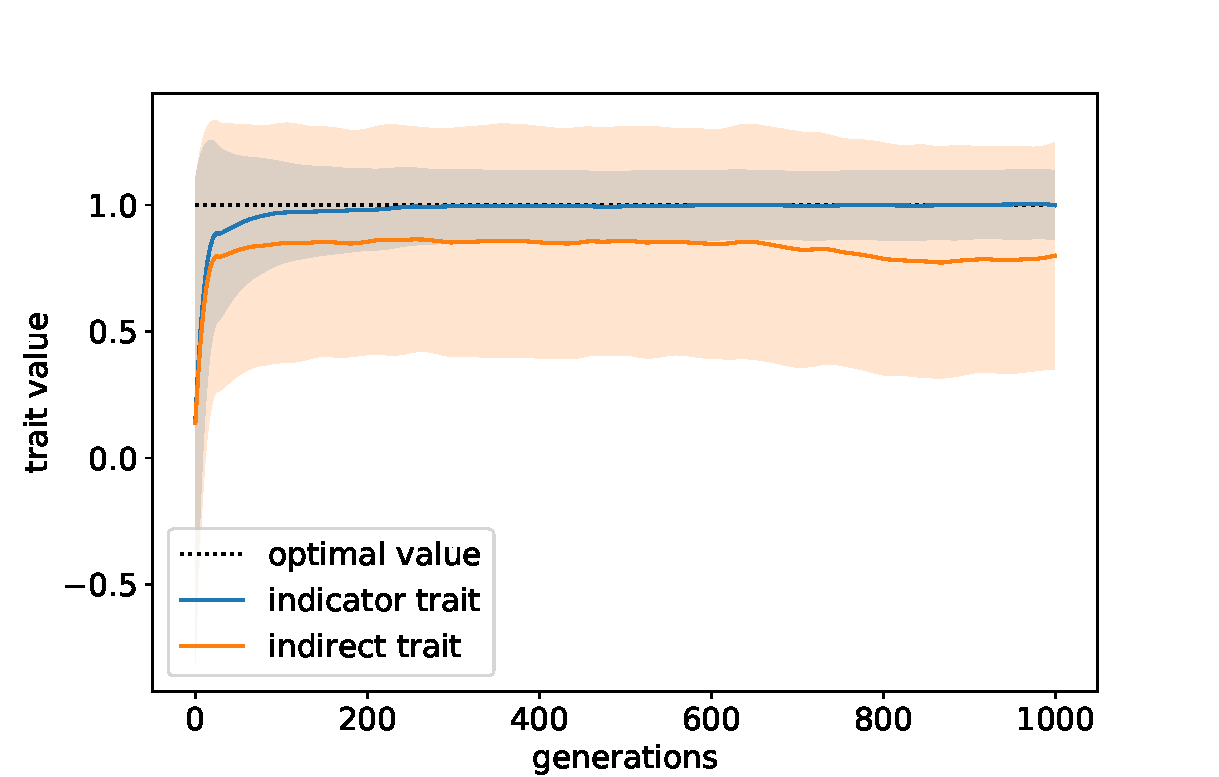
\includegraphics[width=\linewidth]{../../graphs/basic_influence/5000_1000_33_100es_09tc.pdf}
  \caption{Basic influence model. Population size 5000. Mean values of 35 simulations, initial trait values chosen from a 2D normal distribution with a 0.9 correlation. Faded area represents mean of standard deviation}
  \label{basic influence fig}
\end{wrapfigure}
  
 \paragraph*{Aim 3: increasing our model's realisticness by adding horizontal transmission.}\label{horizontal model}
 We believe that in reality, individuals often copy from their own peers, so we create a model that allows a basic form horizontal transmission.
 We think that with horizontal transmission our model is more realistic than a simple non-overlapping model.
 Therefore, we allow horizontal transmission, in addition to oblique transmission, to see how it affects the convergence pace of the traits to a stable value. %allow horizontal
  Here, every copier becomes an available role model instantly after being informed, so its peers could copy from it as well. % horizontal
  The influence is now a recursive equation, contrary to the simple counter it was in the previous step. %influence is recursive
  Once all the copiers are informed, the older generation disappears, and the process is repeated. %repetition
  We expect that the maximum influence value in every generation will be higher than the model with oblique transmission only.
  We also expect that the high influence will slow down the convergence of the traits to the optimum value, and perhaps increase the variance even more. 
 
 \paragraph*{Aim 4: creating a more realistic model by including natural selection and overlapping generations.}\label{cyclic model}
 In some populations, the transmission model of non-overlapping generations may not be realistic enough.
 We therefore define a model that allows an individual to be copied by many generations, same as a village elder that may pass on its knowledge up to 3 generations after his own.  
 Consider a population of $N$ individuals, all born with random indicator and indirect trait values as before. %cyclic model in general
 Every cycle (time unit), one naive individual is born and chooses a role model, he becomes an available role model itself. %process
 In order to bring our model closer to reality, we will add dynamics of \textit{natural selection} by biasing the chance of death with the value of the indirectly biased trait.
 Every $d$ cycles ($d$ could be one cycle), $k$ role models "die", depending on several parameters (we assume $k << N$): %death process
  \textbf{number of cycles alive}: the longer it lived, the greater the chance it would die, i.e dies of old age; %age
  \textbf{random misfortune}: a random value drawn at the moment of evaluation, i.e chance to die in an accident; %random
   \textbf{natural selection}: the indirect trait is either favoured or disfavoured by natural selection. %natural selection
 The death score $D_i$ of role model $i$ is given by:
  \begin{equation}
  D_i = r + a_i + s*B_i,
  \end{equation}
  where $r$ is \textit{random misfortune}: a random normal variable drawn at the moment of evaluation. $a_i$ is the "age" (i.e number of cycles alive), and $s$ is the strength of natural selection where $B_i$ is the indirect trait value. %equation explained
  The probability of role model $i$ to die is given by:
  \begin{equation}
  P_d(i) = \frac {D_i}{\sum\limits_{j=1}^{m} D_j},
  \end{equation}  
   where $m$ is the number of current available role models. 
  We expect that the higher $d$ (number of cycles before death), and the lower the $k$, the maximum influence per cycle will increase.
  We also expect that when the correlation between the indicator and indirect traits is high ($\chi > 0.7$), and natural selection disfavours the optimal indicator trait value ($\hat{A}$). 
  Then the indirect and indicator traits will both still converge to the optimal value, given natural selection is weak enough, therefore decreasing the mean fitness of the population, i.e a \textit{runaway process}.

\section*{Conclusion}
Cultural transmission is the phenomenon of which cultural elements, in the form of attitudes, values, beliefs, and behavioural patterns, are transmitted. %what is cultural transmission
Some cultural traits can be more likely to be copied by others, regardless of their frequency in the population.  %what are the biases
Such transmission biases are common in cultural transmission processes. %agreed by many
Many models are based on the assumption that success can be correctly identified, and easily copied. %many are success biases
Here we assume that success isn't correctly identified, therefore individuals may use other indicators to try and estimate the success of others. %  we disagree, we study prestige
We believe, as \citet{complexityPaper} suggest, that \textit{prestige biases} are more common in nature than success biases, since estimating success is probably harder. %what we propose
We believe prestige is composed of two main components: a trait that indicates success (but doesn't guarantee it), and the influence the individual already has on others. % what is prestige here
We created a model for \textit{prestige bias}, following the \textit{indirect bias} model \citet{evolutionBook} have suggested, and added the \textit{influence trait} to it. %indirect bias
We believe that in this era of social media and "likes" and "tagging" it is even easier than 20 years ago to estimate one's influence over others. %why is it relevant
Hence it is crucial to model the cultural biases more realisticly, and we believe including influence in the definition of prestige bias will help achieve that.
With a more realistic model of a very common cultural transmission bias, we may be able to better understand decision-making processes in humans, including life-changing choices such as occupation or a life partner. 
Our model can be expanded in many ways: observing the effects of different bias functions, including errors in estimating the influence, combining factors of cost when copying from an influential role model (not all could afford to copy from the most popular role model), and analysing the differences when including several optimal values for the indicator trait (multiple preference traits in the population).

\clearpage
\section*{Appendix A - Time table}
\paragraph*{Today - Feb. 2020:} 
We will improve the performance of the simulations, allowing us to test scenarios of larger populations the size of 10,000 or more.
We might reach different conclusions regarding the blending mode transmission, given a considerably larger population.

\paragraph*{Feb - Apr 2020:}
Achieving Aim 2, allowing us to test the effects of \textit{influence} on the population.

\paragraph*{Apr - Jun 2020:}
Achieving Aim 3, allowing us to observe the difference horizontal transmission can cause on the variance and mean value of the traits in the population.

\paragraph*{Jun - Sep 2020:}
Achieving Aim 4, allowing us to observe an increasing force of \textit{influence} on the population, and better understand the effects of it on the mean fitness of the population.

\paragraph*{Sep - Nov 2020:}
Combining the results of the various models into a paper, and submitting for publication.


\clearpage
\bibliography{refs}
\bibliographystyle{apalike}
\end{document}